\documentclass[11pt]{article}
\usepackage[a4paper,margin=1in]{geometry}
\usepackage{amsmath,amssymb,amsthm,mathtools}
\usepackage{booktabs}
\usepackage{enumitem}
\usepackage{float}
\usepackage{graphicx}
\usepackage{hyperref}
\usepackage[nameinlink,capitalise]{cleveref}
\usepackage[numbers,sort&compress]{natbib}

\newtheorem{theorem}{Theorem}[section]
\newtheorem{proposition}[theorem]{Proposition}
\newtheorem{corollary}[theorem]{Corollary}
\newtheorem{remark}[theorem]{Remark}
\newcommand{\norm}[1]{\left\lVert#1\right\rVert}

\title{Block Cross-Column Krylov Gram Certificates\\
\large Preserving Packet Phases in Weighted Stein Tails}
\author{Liang Wang}
\date{July 2026}

\begin{document}
\maketitle

\begin{abstract}
RH-65 showed that a global Lyapunov metric cannot replace peripheral-mode
removal.  The remaining route is to project first and weight only the final
localized residual.  Existing RH-62--RH-64 certificates were vector-valued,
however, while the phase-aware Schur construction of RH-58--RH-60 is a
cross-column Gram problem.  Applying a positive upper to each packet column
separately destroys the cancellation that made the finite-horizon route
effective.

This paper gives a block remedy.  For an isometry $V$, block source
$Z=VB+E$, projected matrix $H=V^*AV$, and Galerkin residual $R=AV-VH$, we
prove the exact identity
\[
 A^LZ=VH^LB+
 \sum_{j=0}^{L-1}A^{L-1-j}RH^jB+A^LE.
\]
In a positive metric with contraction $q<1$, the identity yields (i) a
coefficient-aware center-radius certificate retaining all packet phases and
(ii) a positive-semidefinite Gram envelope valid simultaneously for every
coefficient vector.  Both use the cross-column matrices
$(H^jB)^*R^*MR(H^jB)$ before positive majorization.

On a two-column slow-mode cancellation witness at horizon $32$, independent
column bounds lose a factor $2.129\times10^{18}$, whereas the block
directional certificate has gain $1.0000014$.  A 256-bit Arb audit certifies
that the independent-column loss exceeds $10^{18}$.  On a nonnormal
four-step chain, one block level reduces the gain from $11.37$ to $3.90$ and
rank-four closure is exact.  A six-mode complex-phase model improves from
$1.713$ to $1.288$ before exact rank-six closure.  The uniform PSD envelope
still has gain $410$ in the specially cancelling direction, exposing the next
gate: coefficient-adapted positive residual geometry.  No production block
depth theorem, Stage A1 closure, arithmetic trace formula, or Hilbert--Polya
conclusion is claimed.
\end{abstract}

\noindent\textbf{Keywords:} block Krylov method; cross Gramian; phase
cancellation; Lyapunov metric; Stein tail; packet fusion.

\medskip
\noindent\textbf{MSC 2020:} 47A10; 47B65; 65F35; 93B07; 93D05.

\section{Introduction}

The directional Hardy route is intrinsically multi-source.  Schur packets
produce columns $z_1,\ldots,z_r$ and a coefficient vector $a$; the physical
quantity is the norm of the coherent sum $Za$, not the sum of the packet
norms.  RH-58 kept this information in a time-ordered cross Gram, while
RH-60 retained it over a finite horizon.  The terminal estimates of
RH-62--RH-64 then returned to one source vector
\citep{WangSchurGram2026,WangWeightedResidual2026}.

RH-65 determines the proper order: peripheral or reached slow directions
must be removed before a terminal metric is applied
\citep{WangMetricConditioning2026}.  To transfer that order to packets, the
projection must be block-valued.  Block Krylov spaces are standard for
multiple right-hand sides \citep{Saad2003}; the point here is a specific
positive Gram certificate that does not scalarize the columns prematurely.

\subsection*{Contributions and boundary}

\begin{enumerate}[leftmargin=2.2em]
 \item We prove a block Galerkin power identity with an explicit source
       reconstruction residual.
 \item We derive a directional center-radius certificate and a uniform PSD
       Gram envelope in a Lyapunov metric.
 \item We identify exact cancellation and invariant-block closure criteria.
 \item We audit three finite models and isolate the gap between a selected
       physical direction and one envelope valid for all directions.
\end{enumerate}

All matrix theorems below are finite-dimensional.  The model calculations
are deterministic binary64 evidence; only the displayed cancellation witness
has a 256-bit interval audit.

\section{Block power identity}
\label{sec:identity}

Let $A\in\mathbb C^{n\times n}$, $Z\in\mathbb C^{n\times r}$, and let
$V\in\mathbb C^{n\times k}$ satisfy $V^*V=I$.  Define
\begin{equation}
 B=V^*Z,\qquad E=Z-VB,\qquad
 H=V^*AV,\qquad R=AV-VH.
 \label{eq:block-data}
\end{equation}
For a block Krylov basis, $V$ spans a numerical approximation to
$\operatorname{span}\{Z,AZ,\ldots,A^{d-1}Z\}$, but the next identity does
not require that construction.

\begin{proposition}[Block Galerkin power identity]
\label{prop:power}
For every integer $L\ge0$,
\begin{equation}
 A^LZ=Y_L+\mathcal R_L,
 \qquad Y_L=VH^LB,
 \label{eq:center}
\end{equation}
where
\begin{equation}
 \mathcal R_L=
 \sum_{j=0}^{L-1}A^{L-1-j}RH^jB+A^LE.
 \label{eq:block-remainder}
\end{equation}
\end{proposition}

\begin{proof}
The relation $AV=VH+R$ implies by induction
\[
 A^LVB=VH^LB+\sum_{j=0}^{L-1}A^{L-1-j}RH^jB.
\]
Add $A^LE$ and use $Z=VB+E$.
\end{proof}

The identity keeps every source column inside $B$ and $H^jB$.  No triangle
inequality has yet been applied across packets.

\section{Cross-column weighted certificates}
\label{sec:certificate}

Let $M\succ0$ and suppose
\begin{equation}
 q=\norm{M^{1/2}AM^{-1/2}}_2<1.
 \label{eq:metric-contraction}
\end{equation}
The canonical equation $M-A^*MA=I$ is one sufficient construction
\citep{ZhouDoyleGlover1996}.  Put
\begin{equation}
 Q=R^*MR,qquad Q_E=E^*ME,qquad C_j=H^jB.
 \label{eq:residual-grams}
\end{equation}

\begin{theorem}[Directional block center-radius certificate]
\label{thm:directional}
For every $a\in\mathbb C^r$,
\begin{equation}
 \norm{A^LZa}_M
 \le \norm{Y_La}_M+\rho_L(a),
 \label{eq:directional-upper}
\end{equation}
where
\begin{equation}
 \rho_L(a)=
 \sum_{j=0}^{L-1}q^{L-1-j}
 \sqrt{a^*C_j^*QC_ja}
 +q^L\sqrt{a^*Q_Ea}.
 \label{eq:directional-radius}
\end{equation}
Consequently
\begin{equation}
 a^*(A^LZ)^*M(A^LZ)a
 \le\left(\sqrt{a^*Y_L^*MY_La}+\rho_L(a)\right)^2.
 \label{eq:directional-energy}
\end{equation}
\end{theorem}

\begin{proof}
Apply \eqref{eq:metric-contraction} to each propagated term in
\eqref{eq:block-remainder}.  Since
$\norm{RC_ja}_M^2=a^*C_j^*QC_ja$, the triangle inequality gives
\eqref{eq:directional-upper}; squaring gives
\eqref{eq:directional-energy}.
\end{proof}

For a certificate valid for every coefficient simultaneously, choose
positive weights satisfying
\[
 \theta_0+\cdots+\theta_{L-1}+\theta_E=1,
\]
and define
\begin{equation}
 \mathcal C_L(\theta)=
 \sum_{j=0}^{L-1}
 \frac{q^{2(L-1-j)}}{\theta_j}C_j^*QC_j
 +\frac{q^{2L}}{\theta_E}Q_E.
 \label{eq:residual-envelope}
\end{equation}

\begin{theorem}[Uniform PSD Gram envelope]
\label{thm:gram}
The residual and full block Grams obey
\begin{align}
 \mathcal R_L^*M\mathcal R_L
 &\preceq \mathcal C_L(\theta),
 \label{eq:residual-loewner}\\
 (A^LZ)^*M(A^LZ)
 &\preceq
 (1+\eta)Y_L^*MY_L+(1+\eta^{-1})\mathcal C_L(\theta)
 \label{eq:full-loewner}
\end{align}
for every $\eta>0$.
\end{theorem}

\begin{proof}
For a fixed $a$, apply the weighted Cauchy inequality
$(\sum_i x_i)^2\le\sum_i x_i^2/\theta_i$ to the summands in
\eqref{eq:directional-radius}.  This proves
$\norm{\mathcal R_La}_M^2\le a^*\mathcal C_L(\theta)a$ for every $a$, which
is \eqref{eq:residual-loewner}.  The operator Young inequality
\[
 (X+W)^*(X+W)\preceq
 (1+\eta)X^*X+(1+\eta^{-1})W^*W
\]
with $X=M^{1/2}Y_L$ and $W=M^{1/2}\mathcal R_L$ then gives
\eqref{eq:full-loewner}.
\end{proof}

The implementation chooses trace-optimal scalar weights:
\begin{equation}
 \theta_j\propto q^{L-1-j}
 \sqrt{\operatorname{tr}(C_j^*QC_j)},
 \qquad
 \theta_E\propto q^L\sqrt{\operatorname{tr}Q_E},
 \label{eq:trace-weights}
\end{equation}
and then
$\eta=\sqrt{\operatorname{tr}\mathcal C_L/
\operatorname{tr}(Y_L^*MY_L)}$.  These choices minimize the traces of the
two successive positive envelopes.  They need not be optimal for a selected
coefficient direction.

\begin{corollary}[Exact fused cancellation]
\label{cor:cancellation}
If a coefficient vector $a$ satisfies
\begin{equation}
 Ea=0,qquad RH^jBa=0\quad(0\le j<L),
 \label{eq:annihilation}
\end{equation}
then $\rho_L(a)=0$ and the directional certificate is exact.  This may hold
even when none of the individual source columns has zero residual.
\end{corollary}

\begin{proof}
Every quadratic term in \eqref{eq:directional-radius} vanishes.
\end{proof}

If $E=R=0$, the block subspace is invariant and both certificates are exact
for all coefficient vectors.

\section{Finite-model audit}
\label{sec:audit}

The code builds $V$ by an SVD of the block Krylov matrix and uses the
canonical Lyapunov metric.  Four uppers are compared: the directional block
certificate, the uniform PSD Gram evaluated in the physical direction,
independent scalar-column certificates followed by Minkowski, and a
rank-matched Krylov certificate built only after fusing the selected source.

\begin{table}[H]
\centering
\caption{One-level directional energy gains.}
\label{tab:gains}
\begin{tabular}{lrrrrr}
\toprule
model & rank & block dir. & PSD Gram & independent & fused\\
\midrule
cancelling slow pair & 2 & 1.000001 & 410.159 & $2.129\times10^{18}$ & 1.000000\\
nonnormal chain      & 3 & 3.899145 & 3.950049 & 11.3650 & 5.007690\\
complex phase packets& 3 & 1.288471 & 1.295052 & 1.71263 & 1.129739\\
\bottomrule
\end{tabular}
\end{table}

The cancellation witness has
\[
 A=\operatorname{diag}(0.995,0.55,0.2),\qquad
 Z=\begin{pmatrix}1&-1\\1&1\\0.2&-0.2\end{pmatrix},\qquad
 a=\binom11.
\]
Thus $Za=2e_2$: the slow and fast components cancel before propagation.
The block space contains the invariant fused direction and satisfies
\cref{cor:cancellation}; floating-point orthogonalization leaves only a
$1.4\times10^{-6}$ relative gain.  Separate columns must each carry the
$0.995$ mode and therefore lose more than eighteen orders of magnitude.  A
256-bit Arb calculation certifies the cancellation, positivity of the exact
fused energy, residual annihilation on the fused axis, and an independent-
column lower loss exceeding $10^{18}$.

The same example reveals a distinction.  The trace-global PSD envelope must
also cover coefficient vectors that do not cancel the slow mode, so its
evaluation at $a=(1,1)$ still has gain $410$.  The theorem is valid; the
choice of one global positive envelope is geometrically mismatched to a
special physical direction.

\begin{figure}[H]
\centering
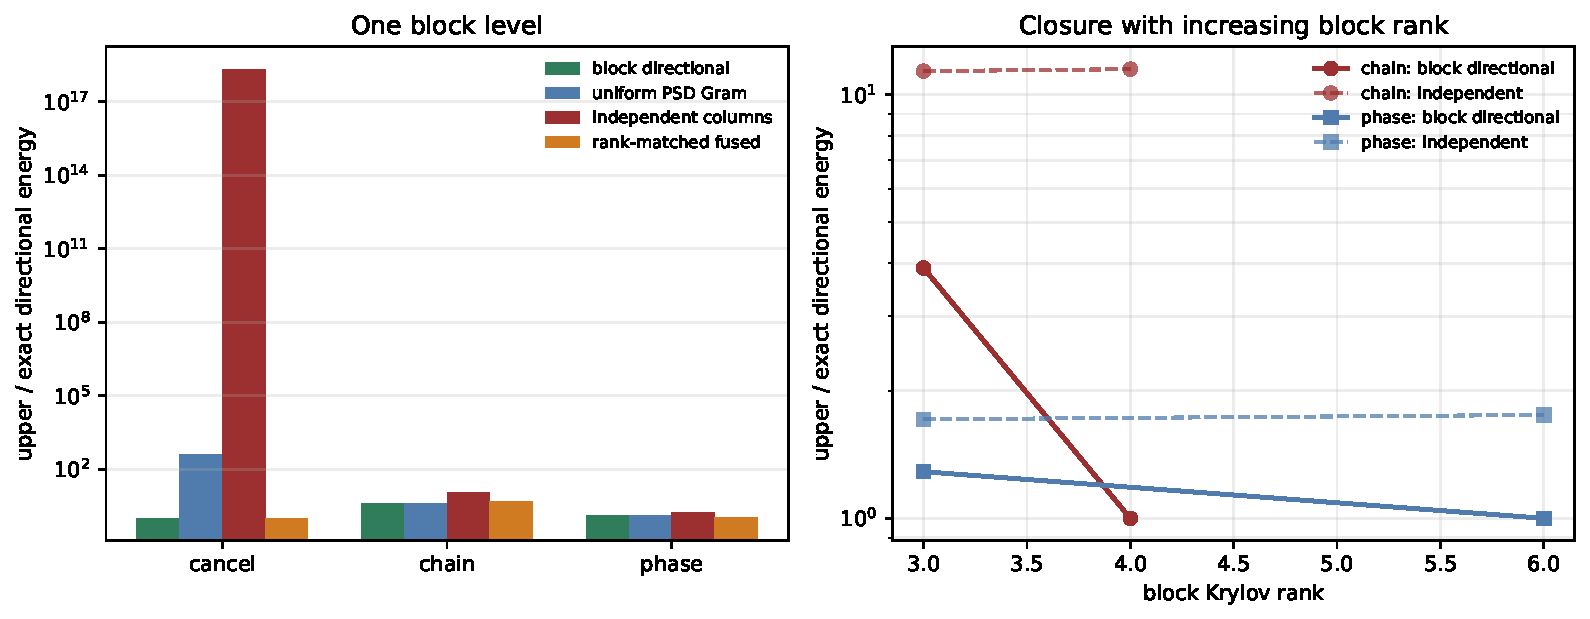
\includegraphics[width=0.98\textwidth]{figures/block_cross_column_krylov_gram.pdf}
\caption{Left: one-level gains, including the catastrophic independent-column
loss in the cancellation witness.  Right: increasing block rank closes the
nonnormal and complex-phase models, while independent scalarization retains
a packet-fusion penalty.}
\label{fig:audit}
\end{figure}

For the nonnormal chain, rank three improves the directional gain from the
independent value $11.37$ to $3.90$; rank four is exact.  For the six-mode
phase model, rank three improves $1.713$ to $1.288$ and rank six is exact.
The minimum eigenvalues of the numerical PSD slack are nonnegative up to
$4.4\times10^{-18}$ rounding.

\section{Route consequence}
\label{sec:route}

RH-66 repairs the cross-column scalarization loss.  The viable terminal
architecture is now
\begin{equation}
 \text{block Krylov center}
 \longrightarrow \text{coherent physical coefficient}
 \longrightarrow \text{localized weighted residual}.
 \label{eq:architecture}
\end{equation}
For a fixed physical coefficient, \cref{thm:directional} can be nearly exact
even when every columnwise estimate fails.

The unresolved question is stronger: Stage A1 ultimately needs a positive
object that can be transferred through packet and continuum limits.  The
trace-global Young envelope in \cref{thm:gram} can overpay for coefficient
directions irrelevant to the physical fusion.  The next gate is therefore a
weighted block residual stress test comparing directional, low-rank cone,
and full PSD formulations.  It must determine how much positivity is truly
needed by the downstream determinant argument.

\section{No arithmetic or Hilbert--Polya conclusion}

This paper constructs no self-adjoint operator, no $T\log T$ counting law,
no prime-power trace formula, and no completed-zeta identity.  It makes no
Hilbert--Polya or Riemann-hypothesis claim.  Stage A1 and unconditional Stage
A4 remain open.

\section{Reproducibility}

The directory contains block algebra, tests, the model pilot, Arb audit,
figures, hashes, and publication artifacts.  The principal commands are:
\begin{verbatim}
pytest -q -p no:cacheprovider
python experiments/run_block_gram_pilot.py
python experiments/run_arb_cancellation_audit.py
MPLBACKEND=Agg python experiments/make_figures.py
latexmk -pdf -interaction=nonstopmode -halt-on-error main.tex
\end{verbatim}

The block identities and positive envelopes are analytic.  The model gains
are binary64 evidence.  Uniform physical-family block depth, interval-
certified production packet transfer, Stage A1, unconditional Stage A4, a
self-adjoint Hilbert--Polya operator, an arithmetic trace formula, and a
zeta-zero identity remain open.

\bibliographystyle{plainnat}
\bibliography{references}
\end{document}
